\documentclass{beamer}

\usepackage[english]{babel}

\usepackage[latin1]{inputenc}

\usepackage{times}
\usepackage{hyperref}
\usepackage{listings}
\usepackage{comment}
\usepackage{booktabs} % for toprule
\usepackage{tikz}
\usetikzlibrary{positioning}

\lstset{frame=none, showstringspaces=false, basicstyle=\footnotesize,
  xleftmargin=-8mm,language=Haskell}

\newcommand{\colAwidth}{0.1\textwidth}
\newcommand{\colBwidth}{0.8\textwidth}

\title[GOOL]{Multi-lingual code generation in Drasil}

\author{\underline{Jacques Carette}, Spencer Smith, Dan Szymczak and
Steven Palmer}

\institute[McMaster University]{McMaster University}

\date[July 2017]{WG 2.11, July 2017 Meeting}

\beamertemplatenavigationsymbolsempty 

\begin{document}

%I will present some ongoing work that seeks to generate all the artefacts
%involved in software (obviously code, but also specification documents, design
%documents, tests, user manual, Makefiles, etc). In the context of software
%which requires (re)certification, all of these artefacts are involved -- and
%they normally contain a huge amount of duplicate information. Our approach is
%to do very aggressive knowledge encapsulation, followed by relatively
%straightforward generation passes. For domains (such as scientific computation)
%where there is well-established theory, our preliminary experiments shows that
%this works quite well. Note that we do NOT expect this to work so well in
%domains without well-established theory.

\begin{frame}
\titlepage
\end{frame}

\begin{frame}

\includegraphics{generate_all_the_things.jpg}
\end{frame}

\begin{frame}

\includegraphics[width=\textwidth]{no_silver_bullet.jpg}
\end{frame}

\begin{frame}
\frametitle{Context}
{\Large software \onslide<2->{(re)}certification}
\vspace*{.2cm}
\begin{itemize}
\item<3->All software artefacts as \textcolor{green}{evidence}:
\begin{itemize}
\item \textcolor{blue}{requirements, software specification, software design, code, 
  tests, ``theory manual'', user manual, \ldots}
\end{itemize}
\vspace*{.5cm}
\item<4->Massive amounts of \textcolor{red}{knowledge duplication}
\begin{itemize}
  \item Implies that either
  \begin{itemize}
    \item non-code artefacts do not get maintained well enough, OR
    \item are felt to be an expensive nuisance
  \end{itemize}
  \item duplication harms traceability
\end{itemize}
\end{itemize}
\vfill
\end{frame}

\begin{frame}[t]
\frametitle{Ontologies}
\only<4>{\framesubtitle{Language Concepts}}
{\large \onslide<1-3,5->{\only<1-2>{\color{blue}}Data.Drasil} 
\onslide<3,5->{- \only<3>{\color{blue}}Language Concepts}
\onslide<5->{- \only<5->{\color{blue}}Document Language}}

\only<2>{
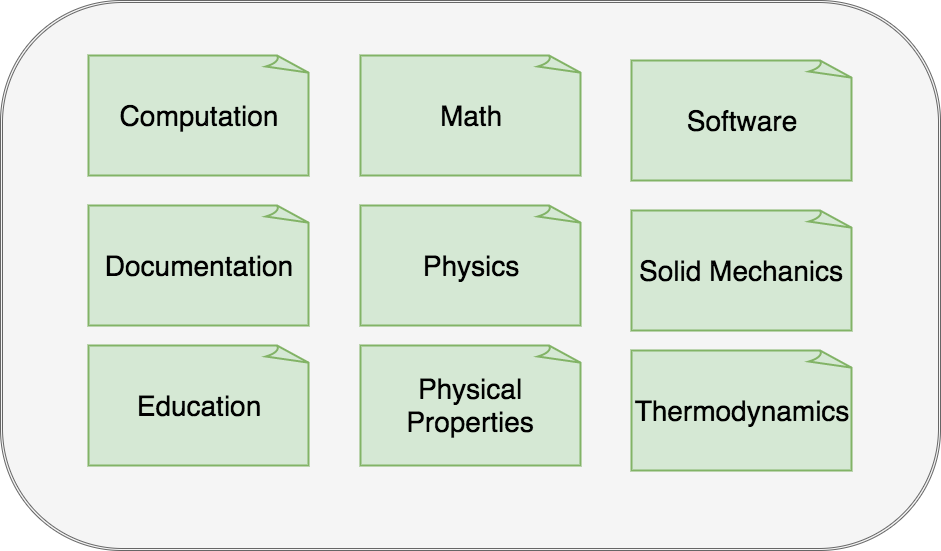
\includegraphics[scale=0.25]{Data_Drasil.png}
}
\only<4>{
\center{\vspace{-1cm}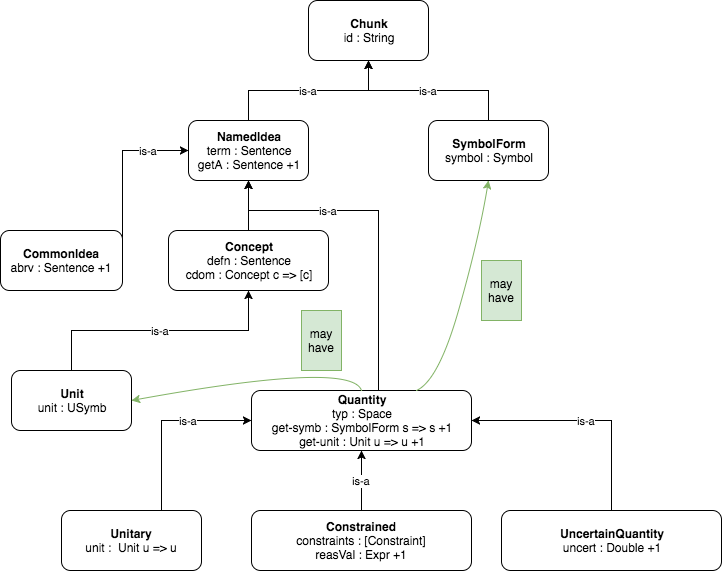
\includegraphics[scale=0.37]{class_hierarchy.png}}
}
\only<6>{
\vspace{2cm}
\emph{\Large{See Code}}
%\begin{enumerate}
%\item \emph{Recipe} language
%\item Multiple little languages
%\end{enumerate}
}
\end{frame}

\begin{frame}
  \frametitle{Example (GlassBR)
(see documents and code)}
\end{frame}

% Drasil
%%% - generate all the things
%%% - no silver bullet
%%% - context
% * example: doc (D) + code (S) (GlassBR)
% - ontologies (D)
%   * go through well-formatted Data.Drasil.Concepts.*, Data.Drasil.SI_Units
%       (D - if you could make sure these are as clean as possible?)
%   - typeclasses of Language.Drasil (D) [esp. as this has evolved a lot recently]
%   * Example.Drasil.DocumentLanguage.
% 
% Gool
% - origins (J)
% - design
%   - meta-language abstracting details (J)
%     - all required features of all languages (S?)
%        ex: public/private
%     - 7 language renderers (as virtual dispatch table - in Haskell!) (S)
%     - pretty-printer to make things look nice
%     - lots of smart constructors to make it look PL-like (give example) (S)
% 
% Choices
% - implementation choices, design choices, "aspects" (J)
% - examples of
%   - implementation choices (S)
%   - design choices (S) 

%%%%%%%%%%%%%%%%%%%%
%
% things to think about
%
% We have 3 completely differents means of information capture (Data.Drasil.*
% chunks; Drasil language concepts via classes; DocumentLanguage).  But all 3
% capture 'domain information'.  But used in different ways.  The chunks are
% mostly noun-like data, the classes represent a meta-model of the data, and the
% DocumentLanguage is executable.  [It can, and likely eventually will, be made
% into chunks too].

\end{document}

\begin{frame}
\frametitle{Literate Programming}
What can we learn from it?
\begin{enumerate}
\item<2-> Code in most languages is not well organized for 
  \textcolor{red}{human understanding}.
\item<3-> Code in some languages can not \textcolor{red}{efficiently} be broken 
down into very small pieces.
\item<4-> Chunk labels add convenient \textcolor{red}{traceability} information.
\end{enumerate}
\vfill
\end{frame}

\begin{frame}
\frametitle{Drasil}
Ideas behind our prototype:
\begin{enumerate}
\item<1-> \textcolor{red}{no information duplication}
\item<2-> \textcolor{red}{Recipes} used to weave together information into
documents / software artefacts.
\end{enumerate}
\vspace*{1cm}
\onslide<3->{Implies:}
\begin{itemize}
\item<3-> Bug in one place, bugs everywhere!
\item<4-> Huge up-front investment.
\item<5-> Doesn't work if you have no theory.
\end{itemize}
\vfill
\end{frame}

\begin{frame}
\frametitle{Example (high level)}
\begin{center}
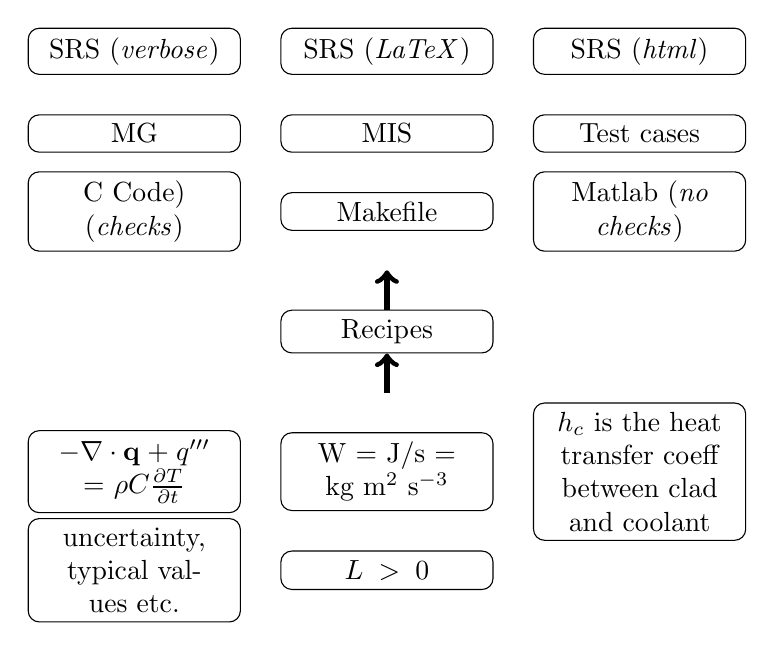
\begin{tikzpicture}[node distance=5mm]
  \tikzstyle{every node}=[draw,shape=rectangle, rounded corners,
    text width=7em, text centered];
  \node (srs)                     	{SRS (\emph{LaTeX})};
  \node (srsh) [right = of srs]  {SRS (\emph{html})};
  \node (srsv) [left = of srs] 	{SRS (\emph{verbose})};
  \node (mis) [below = of srs]       {MIS};
  \node (mg) [left = of mis]       {MG};
  \node (test) [right = of mis]       {Test cases};
  \node (make) [below = of mis]       {Makefile};
  \node (code) [left = of make]       {C Code) (\emph{checks})};
  \node (matlab) [right = of make]       {Matlab (\emph{no checks})};
  \node (recipes) [below = 10mm of make]       {Recipes};
  \node (units) [below = 10mm of recipes]       {W = J/s = kg m$^2$ s$^{-3}$};
  \node (eq) [left = of units]       {$-{\bf \nabla \cdot q} +q'''$ = $\rho C \frac{\partial T}{\partial t}$};
  \node (descipt) [right = of units]       {$h_c$ is the heat transfer coeff between clad and coolant};
  \node (constraint) [below = of units]       {$L > 0$};
  \node (know) [left = of constraint]       {uncertainty, typical values etc.};

  \draw [shorten <=5mm, <-, line width=2pt] (make) -- (recipes);
  \draw [shorten <=5mm, ->, line width=2pt] (units) -- (recipes);
\end{tikzpicture}
\end{center}
\end{frame}

\begin{frame}
\frametitle{Sanity checks}
\begin{table} 
\centering
%\caption{Constraints on quantities}
\begin{tabular}{c c r c } 
\toprule
\textbf{Var} & \textbf{Constraints} & \textbf{Typical Value} & \textbf{Uncertainty}\\ \midrule
$L$ & $L > 0$ & 1.5 m & 10\% \\ 
$D$ & $D > 0$ & 0.412 m & 10\% \\ 
$V_P$ & $V_P > 0$ & 0.05 m$^3$	& 10\% \\
$A_P$ & $A_P > 0$ & 1.2 m$^2$	& 10\% \\
$\rho_P$ & $\rho_P > 0$	& 1007 kg/m$^3$	& 10\% \\
\bottomrule
\end{tabular}
\label{tab:pcm}
\end{table}

\begin{equation*}
E_W = \int_{0}^{t} h_C A_C (T_C - T_W(t)) dt - \int_{0}^{t} h_P A_P (T_W(t) - T_P(t)) dt
\end{equation*}

\begin{itemize}
\item Sanity checks captured and reused
\item Generate guards against invalid input
\item Generate test cases
\end{itemize}
\end{frame}

\begin{frame}
\frametitle{Reusability}
\noindent
\begin{minipage}{\columnwidth}
\begin{tabular}{@{} p{\colAwidth}  p{\colBwidth}@{}}
\toprule
\textbf{Ref}& \textbf{T1} \\
\midrule
Label &\bf Conservation of energy\\
\midrule
Eq &  $-{\bf \nabla \cdot q} +q'''$ = $\rho C \frac{\partial T}{\partial t}$ \smallskip\\
\midrule
Desc. & Conservation of energy for time varying heat transfer in a material of
specific heat capacity $C$ and density $\rho$, where $\bf q$ is the thermal
flux vector, $q'''$ is the volumetric heat generation, $T$ is the temperature,
$\nabla$ is the del operator and $t$ is time.\\
\bottomrule
\end{tabular}
\end{minipage}
\end{frame}

\begin{frame}
\frametitle{Basic Drasil Design}
\begin{center}
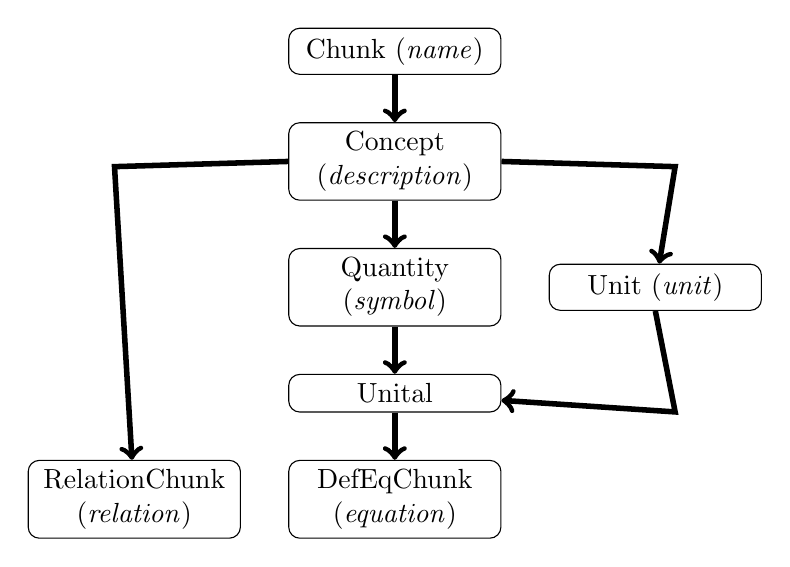
\begin{tikzpicture}[node distance=6mm]
  \tikzstyle{every node}=[draw,shape=rectangle, rounded corners,
    text width=7em, text centered];
  \node (ch)                     	{Chunk (\emph{name})};
  \node (co) [below = of ch]       {Concept (\emph{description})};
  \node (qu) [below = of co]  		{Quantity (\emph{symbol})};
  \node (u ) [right = of qu] 		{Unit (\emph{unit})};
  \node (uc) [below = of qu] 		{Unital};
  \node (eq) [below = of uc]	{DefEqChunk (\emph{equation})};
  \node (rc) [left = of eq]	{RelationChunk (\emph{relation})};

  \draw [->, line width=2pt] (ch) -- (co);
  \draw [->, line width=2pt] (co.west) -- (-3.56,-1.465) -- (rc); 
		%No idea how to do this
  \draw [->, line width=2pt] (co) -- (qu);
  \draw [->, line width=2pt] (co.east) -- (3.56,-1.465) -- (u );
  \draw [->, line width=2pt] (qu) -- (uc);
  \draw [->, line width=2pt] (u .south) -- (3.56,-4.58) -- (uc);
  \draw [->, line width=2pt] (uc) -- (eq);
\end{tikzpicture}
\end{center}
\end{frame}

\begin{frame}[plain, fragile]
\frametitle{Example Recipe}
\vspace*{-8mm}
\begin{lstlisting}
vars :: [EqChunk]
vars = [h_g, h_c]

s1, s2, s3, s4 :: LayoutObj
s1=table_of_units si_units
s2=table_of_symbols vars
s3=Section 0 (S "Data Definitions") $ map (Definition.Data) vars
s4=Section 0 (S "Code") $ map (CodeBlock.toCode CLang Calc) [h_c]

srs :: Quantity s => [s] -> String -> [LayoutObj] -> Document
srs ls author body =
  Document ((S "SRS for ") :+: 
    (foldr1 (:+:) (intersperse (S " and ") 
    (map (\x -> U $ x ^. symbol) ls))))
    (S author) body  
  
srsBody :: Document
srsBody = srs vars "Spencer Smith" [s1, s2, s3, s4]
\end{lstlisting}
\end{frame}

\begin{frame}[plain, fragile]
\frametitle{Example Recipe}
\begin{lstlisting}
table_of_symbols :: (Unit s, Quantity s) => [s] -> LayoutObj
table_of_symbols ls=Section 0 (S "Table of Sym") [intro,table ls]

table :: (Unit s, Quantity s) => [s] -> LayoutObj
table ls=Table [S "Symbol",S "Description",S "Units"] (mkTable
  [(\ch -> U (ch ^. symbol)), 
   (\ch -> ch ^. descr), 
   (\ch -> Sy $ ch ^. unit)] ls)
  (S "Table of Symbols") False
\end{lstlisting}
\pause
\vspace*{0.6cm}
{\hspace{-4mm}\large\bf Classy Optics}
\begin{lstlisting}
class Chunk c where
  name :: Simple Lens c String
class Chunk c => Concept c where
  descr :: Simple Lens c Sentence
\end{lstlisting}
\end{frame}

\begin{frame}[plain, fragile]
\frametitle{Units Recipe}
\begin{lstlisting}
fundamentals :: [FundUnit]
fundamentals = [metre, kilogram, second,kelvin,mole,ampere,candela]

derived :: [DerUChunk]
derived = [centigrade, joule, watt, calorie, kilowatt]

si_units :: [UnitDefn]
si_units = map UU fundamentals ++ map UU derived

------------- Fundamental SI Units ---------------------------------------------
fund :: String -> String -> String -> FundUnit
fund nam desc sym = UD (CC nam (S desc)) (UName $ Atomic sym)

metre, kilogram, second,kelvin,mole,ampere,candela :: FundUnit
metre    = fund "Metre"    "length"               "m"
kilogram = fund "Kilogram" "mass"                 "kg"
second   = fund "Second"   "time"                 "s"
kelvin   = fund "Kelvin"   "temperature"          "K"
mole     = fund "Mole"     "amount of substance"  "mol"
ampere   = fund "Ampere"   "electric current"     "A"
candela  = fund "Candela"  "luminous intensity"   "cd"

\end{lstlisting}
\end{frame}

\begin{frame}[plain, fragile]
\frametitle{The $h_c$ Chunk}
$$h_{c} = \frac{2k_{c} h_{b}}{2k_{c}+\tau_{c}h_{b}}$$
\begin{lstlisting}
heat_transfer :: DerUChunk
heat_transfer = DUC (UD ht_con ht_symb) heat_transfer_eqn

ht_con :: ConceptChunk
ht_con = makeCC "Heat transfer" "Heat transfer"

ht_symb :: USymb
ht_symb = from_udefn heat_transfer_eqn

heat_transfer_eqn = USynonym (UProd 
  [kilogram ^. unit, UPow (second ^. unit) (-3),
   UPow (centigrade ^. unit) (-1)])

h_c_eq :: Expr
h_c_eq = 2*(C k_c)*(C h_b)/(2*(C k_c)+(C tau_c)*(C h_b))

h_c :: EqChunk
h_c = fromEqn "h_c" (S "convective heat transfer ...") 
  (lH `sub` lC) heat_transfer h_c_eq
\end{lstlisting}
\end{frame}

\begin{frame}
\frametitle{Design Documentation}
\begin{center}
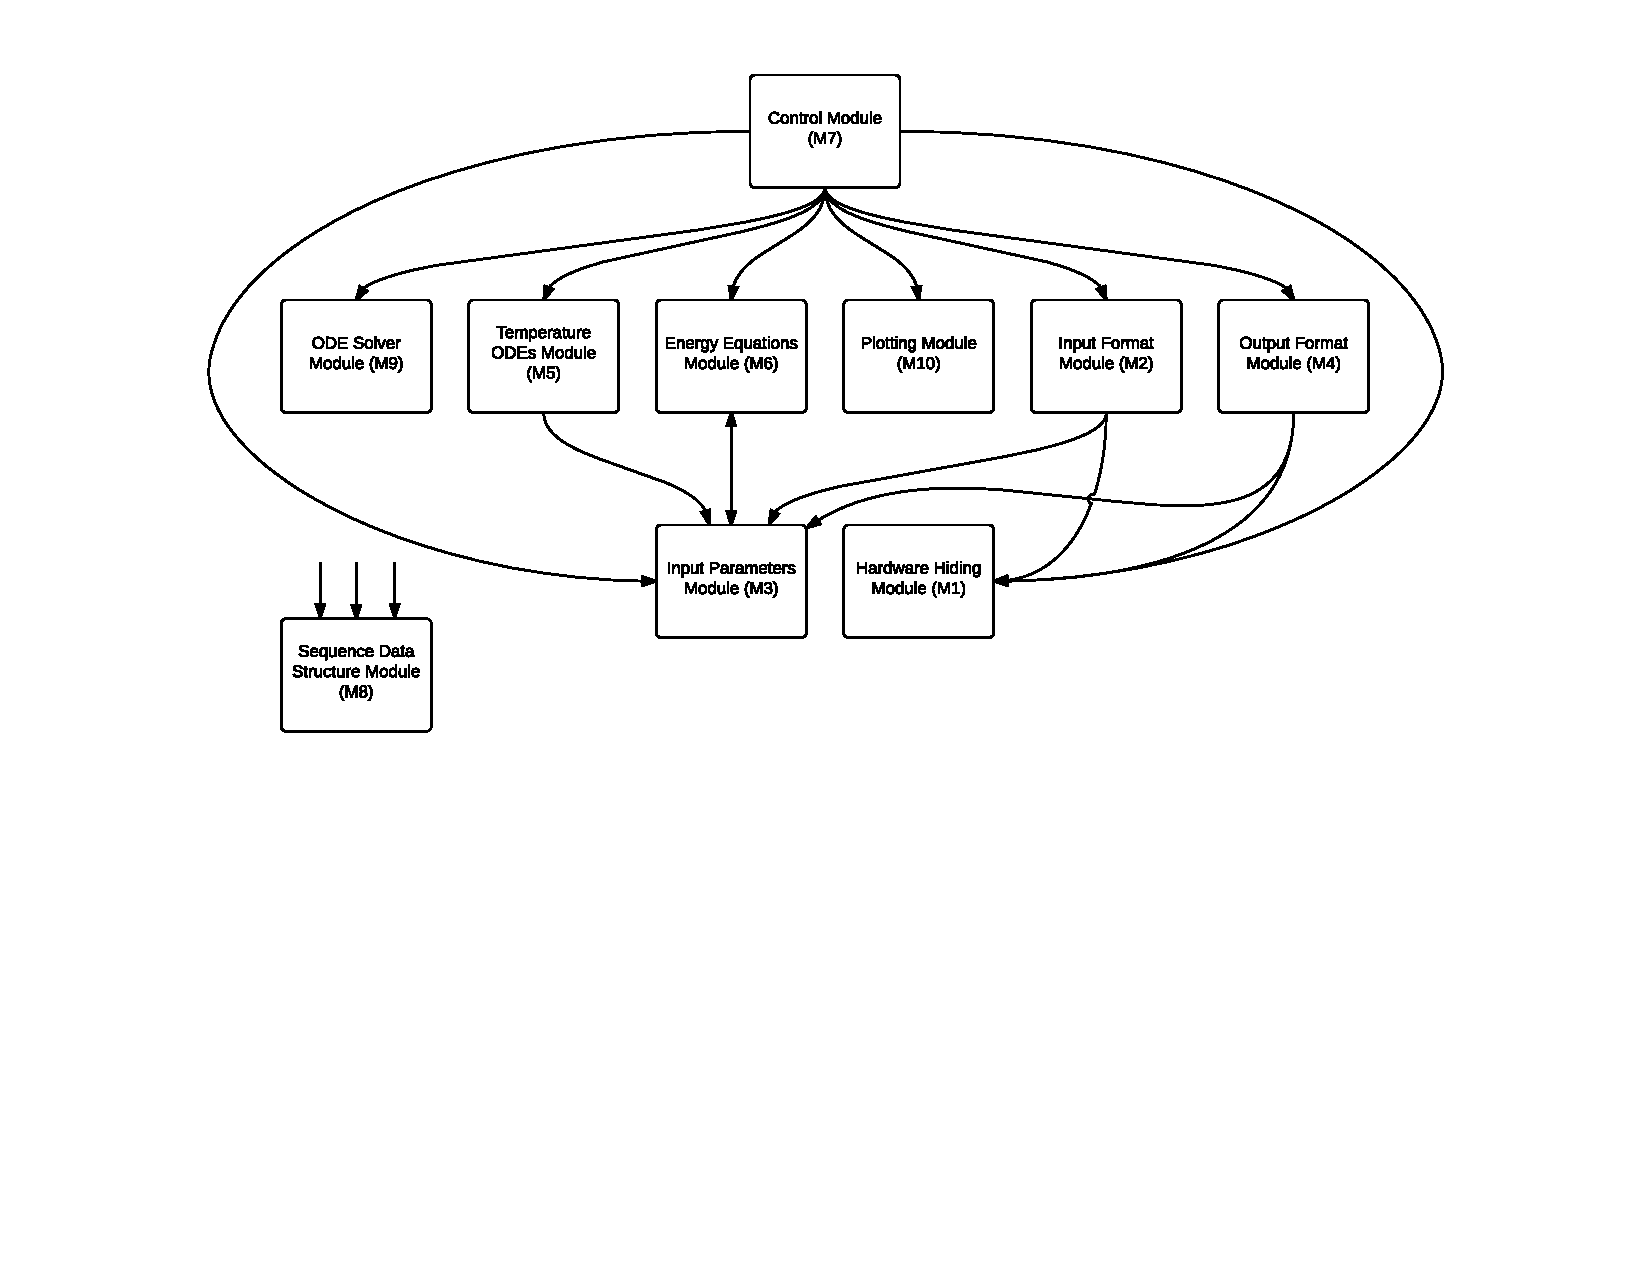
\includegraphics[scale=0.47]{../PASC16/UsesHierarchy.pdf}
\end{center}
\end{frame}

\begin{frame}
\frametitle{Approach}
\begin{itemize}
\item Case studies
\begin{itemize}
\item Solar water heating tank
\item Slope stability analysis
\item Glass safety analysis
\item Game physics engine
\item (medium-sized industrial code)
\end{itemize}
\item Small chunks of knowledge
\item Aggressively look for patterns and capture
\item Currently working on capturing design decisions
\end{itemize}
\pause

\includegraphics[width=0.48\textwidth]{generate_all_the_things.jpg}

\includegraphics[width=0.48\textwidth]{no_silver_bullet.jpg}

\end{frame}

\end{document}
